% Options for packages loaded elsewhere
\PassOptionsToPackage{unicode}{hyperref}
\PassOptionsToPackage{hyphens}{url}
%
\documentclass[
]{article}
\usepackage{lmodern}
\usepackage{amsmath}
\usepackage{ifxetex,ifluatex}
\ifnum 0\ifxetex 1\fi\ifluatex 1\fi=0 % if pdftex
  \usepackage[T1]{fontenc}
  \usepackage[utf8]{inputenc}
  \usepackage{textcomp} % provide euro and other symbols
  \usepackage{amssymb}
\else % if luatex or xetex
  \usepackage{unicode-math}
  \defaultfontfeatures{Scale=MatchLowercase}
  \defaultfontfeatures[\rmfamily]{Ligatures=TeX,Scale=1}
\fi
% Use upquote if available, for straight quotes in verbatim environments
\IfFileExists{upquote.sty}{\usepackage{upquote}}{}
\IfFileExists{microtype.sty}{% use microtype if available
  \usepackage[]{microtype}
  \UseMicrotypeSet[protrusion]{basicmath} % disable protrusion for tt fonts
}{}
\makeatletter
\@ifundefined{KOMAClassName}{% if non-KOMA class
  \IfFileExists{parskip.sty}{%
    \usepackage{parskip}
  }{% else
    \setlength{\parindent}{0pt}
    \setlength{\parskip}{6pt plus 2pt minus 1pt}}
}{% if KOMA class
  \KOMAoptions{parskip=half}}
\makeatother
\usepackage{xcolor}
\IfFileExists{xurl.sty}{\usepackage{xurl}}{} % add URL line breaks if available
\IfFileExists{bookmark.sty}{\usepackage{bookmark}}{\usepackage{hyperref}}
\hypersetup{
  pdftitle={Forecast Similarity Using Cramer Distance Approximation},
  pdfauthor={Johannes Bracher, Evan Ray, Nick Reich, Nutcha Wattanachit},
  hidelinks,
  pdfcreator={LaTeX via pandoc}}
\urlstyle{same} % disable monospaced font for URLs
\usepackage[margin=1in]{geometry}
\usepackage{graphicx}
\makeatletter
\def\maxwidth{\ifdim\Gin@nat@width>\linewidth\linewidth\else\Gin@nat@width\fi}
\def\maxheight{\ifdim\Gin@nat@height>\textheight\textheight\else\Gin@nat@height\fi}
\makeatother
% Scale images if necessary, so that they will not overflow the page
% margins by default, and it is still possible to overwrite the defaults
% using explicit options in \includegraphics[width, height, ...]{}
\setkeys{Gin}{width=\maxwidth,height=\maxheight,keepaspectratio}
% Set default figure placement to htbp
\makeatletter
\def\fps@figure{htbp}
\makeatother
\setlength{\emergencystretch}{3em} % prevent overfull lines
\providecommand{\tightlist}{%
  \setlength{\itemsep}{0pt}\setlength{\parskip}{0pt}}
\setcounter{secnumdepth}{-\maxdimen} % remove section numbering
\usepackage{amsmath}
\usepackage{tabularx}
\usepackage{hyperref}
\usepackage{multicol}
\usepackage{longtable}
\usepackage{array}
\usepackage{multirow}
\usepackage{wrapfig}
\usepackage{float}
\usepackage{colortbl}
\usepackage{pdflscape}
\usepackage{tabu}
\usepackage{threeparttable}
\usepackage{threeparttablex}
\usepackage{makecell}
\usepackage{xcolor}
\usepackage{tikz}
\usepackage{pgfplots}
\ifluatex
  \usepackage{selnolig}  % disable illegal ligatures
\fi

\title{Forecast Similarity Using Cramer Distance Approximation}
\author{Johannes Bracher, Evan Ray, Nick Reich, Nutcha Wattanachit}
\date{03/02/2021}

\begin{document}
\maketitle

\hypertarget{cramer-distance}{%
\section{Cramer Distance}\label{cramer-distance}}

Consider two predictive distributions \(F\) and \(G\). Their
\emph{Cramer distance} or \emph{integrated quadratic distance} is
defined as

\[
\text{CD}(F, G) = \int_{-\infty}^\infty(F(x) - G(x))^2 dx
\] where \(F(x)\) and \(G(x)\) denote the cumulative distribution
functions. It can also be written as \begin{equation}
\text{CD}(F, G) = \mathbb{E}_{F, G}|x - y| - 0.5 \left[\mathbb{E}_F|x - x'| + \mathbb{E}_G|y - y'| \right], \label{eq:formulation_expectations}
\end{equation} where \(x, x'\) are independent random variables
following \(F\) and \(y, y'\) are independent random variables following
\(G\). This formulation illustrates that the Cramer distance depends on
the shift between \(F\) and \(G\) (first term) and the variability of
both \(F\) and \(G\) (of which the two last expectations in above
equation are a measure).

The Cramer distance is the divergence associated with the continuous
ranked probability score (Thorarinsdottir 2013, Gneiting and Raftery
2007), which is defined by

\begin{align}
\text{CRPS}(F, y) &= \int_{-\infty}^\infty(F(x) - \mathbf{1}(x \geq y))^2 dx = ) \\
&= 2\int_0^1((\mathbf{1}(y \leq q^F_k)-\tau_k)(q^F_k-y) d\tau_k \label{eq:crps}
\end{align}

where y denotes the observed value. Indeed, it is a generalization of
the CRPS as it simplifies to the CRPS if one out of F and G is a
one-point distribution. Indeed, it is a generalization of the CRPS as it
simplifies to the CRPS if one out of \(F\) and \(G\) is a one-point
distribution. The Cramer distance is commonly used to measure the
similarity of forecast distributions (see Richardson et al 2020 for a
recent application).

\hypertarget{cramer-distance-approximation-for-equally-spaced-intervals}{%
\subsection{Cramer Distance Approximation for Equally-Spaced
Intervals}\label{cramer-distance-approximation-for-equally-spaced-intervals}}

Now assume that for each of the distributions \(F\) and \(G\) we only
know \(K\) quantiles at equally spaced levels
\(\tau_1 = 1/(K + 1), \tau_2 = 2/(K + 1), \dots, \tau_K = K/(K + 1)\).
Denote these quantiles by \(q^F_1 \leq q^F_1 \leq \dots \leq q^F_K\) and
\(q^G_1 \leq q^G_2 \leq \dots \leq q^G_K\), respectively. It is well
known that the CRPS can be approximated by an average of linear quantile
scores (Laio and Tamea 2007, Gneiting and Raftery 2007):
\begin{equation}
\text{CRPS}(F, y) \approx \frac{1}{K} \times \sum_{k = 1}^K 2\{\mathbf{1}(y \leq q^F_k) - k/(K + 1)\} \times (q^F_k - y).\label{eq:linear_quantile_scores}
\end{equation} This approximation is equivalent to the weighted interval
score (WIS) which is in use for evaluation of quantile forecasts at the
Forecast Hub, see Section 2.2 of Bracher et al (2021). This
approximation can be generalized to the Cramer distance as
\begin{equation}
\text{CD}(F, G) \approx \frac{1}{K(K + 1)}\sum_{i = 1}^K\sum_{j = 1}^K 2 \times \mathbf{1}\{(i \leq j \land q^F_i > q^G_j) \lor (i \geq j \land q^F_i < q^G_j)\} \times \left| q^F_i - q^G_j\right|. \label{eq:approx_cd}
\end{equation} This can be seen as a sum of penalties for
\textit{incompatibility} of predictive quantiles. Whenever the
predictive quantiles \(q_i^F\) and \(q_j^G\) are incompatible in the
sense that they imply \(F\) and \(G\) are different distributions
(because \(q_F^i > q_G^j\) despite \(i \leq j\) or vice versa), a
penalty \(\left| q^F_i - q^G_j\right|\) is added.

\hypertarget{cramer-distance-approximation-for-unequally-spaced-intervals}{%
\subsection{Cramer Distance Approximation for Unequally-Spaced
Intervals}\label{cramer-distance-approximation-for-unequally-spaced-intervals}}

Suppose we have quantiles \(q_{1}^F,...,q_{K}^F\) and
\(q_{1}^G,...,q_{K}^G\) at \(K\) probability levels
\(\tau_1,...,\tau_K\) (with \(\tau_1=0\)) from two distributions \(F\)
and \(G\). Define the combined vector of quantiles
\(q_1, . . . , q_{2K}\) by combining the vectors \(q_{1}^F,...,q_{K}^F\)
and \(q_{1}^G,...,q_{K}^G\) and sorting them in an ascending order. The
CRPS can be approximated as follows \begin{equation}
\text{CRPS}(F, y) \approx \frac{1}{K}\sum_{k = 1}^K 2\{\mathbf{1}(y \leq q^F_k)-\tau_k\} \times (q^F_k - y) .\label{eq:ls_unqe}
\end{equation}

This approximation can be generalized to the Cramer distance as
\begin{equation}
\text{CD}(F, G) \approx \frac{1}{K}\sum_{i = 1}^K\sum_{j = 1}^K 2 \times w_{ij} \times \mathbf{1}\{(i \leq j \land q^F_i > q^G_j) \lor (i \geq j \land q^F_i < q^G_j)\} \times \left| q^F_i - q^G_j\right|, \label{eq:approx_cd_uneq}
\end{equation}

where \(w_{ij}=|\tau_i-\tau_j|\) (the difference of the probability
levels). The details on how to go from \eqref{eq:approx_cd_uneq} to the
Riemann sums are still being worked out. Essentially, we can approximate
the Cramer distance by eliminating the tails of the integral to the left
of \(q_1\) and the right of \(q_{2K}\), and approximating the center via
a Riemann sum:

\begin{align}
\text{CD}(F,G) &=\int^\infty_{-\infty}{F(x)−G(x)}^2dx\\
&\approx \int^{q_{2K}}_{q_1}{F(x)−G(x)}^2dx\\
&=\sum^{2K-1}_{j=1}\int^{q_{j+1}}_{q_j}{F(x)−G(x)}^2dx
\end{align}

There are a variety of options that can be used for each term in this
sum, for instance:

\hypertarget{left-sided-riemann-sum-approximation}{%
\subsubsection{Left-sided Riemann sum
approximation}\label{left-sided-riemann-sum-approximation}}

\begin{align}
\text{CD}(F,G) &\approx\sum^{2K-1}_{j=1}\int^{q_{j+1}}_{q_j}{F(x)−G(x)}^2\\
&\approx\sum^{2K-1}_{j=1}\{\hat{F}(q_j)-\hat{G}(q_j)\}^2(q_{j+1}-q_{j})\\
\end{align}

Since \(q_j\in \{q_1, ..., q_{2K}\}\) belongs to either
\(q_{1}^F,...,q_{K}^F\) or \(q_{1}^G,...,q_{K}^G\), we can rewrite the
above approximation using \(\tau_1,...,\tau_K\) as follows

\begin{align}
\text{CD}(F,G) 
&\approx\sum^{2K-1}_{j=1}\{\hat{F}(q_j)-\hat{G}(q_j)\}^2(q_{j+1}-q_{j})\\
&=\sum^{2K-1}_{j=1}\{\tau^F_j-\tau^G_j\}^2(q_{j+1}-q_{j})
\end{align}

where \(\tau^F_j \in \boldsymbol{\tau_F}\) and
\(\tau^G_j \in \boldsymbol{\tau_G}\). \(\boldsymbol{\tau_F}\) and
\(\boldsymbol{\tau_G}\) are vectors of length \(2K-1\) with elements

\[
\tau^F_j=
\begin{cases}
I(q_1=q_1^F)\times \tau_{q_1}^F\hspace{7cm}\text{for }j=1\\
I(q_j\in \{q_1^F, ..., q_{K}^F\})\times \tau_{q_j}^F+I(q_j\in \{q_1^G, ..., q_{K}^G\})\times \tau_{j-1}^F\hspace{0.3cm}\text{for }j>1\\
\end{cases}
\]

where \(\tau_{q_j}^F\) is the probability level corresponding to \(q_j\)
given \(q_j\) in the pooled quantiles comes from \(F\), and
\(\tau_{j-1}^F\) is the \((j-1)^{th}\) probability level in
\(\boldsymbol{\tau_F}\).

\[
\tau^G_j=
\begin{cases}
I(q_1=q_1^G)\times \tau_{q_1}^G\hspace{7cm}\text{for }j=1\\
I(q_j\in \{q_1^G, ..., q_{K}^G\})\times \tau_{q_j}^G+I(q_j\in \{q_1^F,...,q_{K}^F\})\times \tau_{j-1}^G\hspace{0.3cm}\text{for }j>1\\
\end{cases}
\]

where \(\tau_{q_j}^G\) is the probability level corresponding to \(q_j\)
given \(q_j\) in the pooled quantiles comes from \(G\), and
\(\tau_{j-1}^G\) is the \((j-1)^{th}\) probability level in
\(\boldsymbol{\tau_G}\).

\hypertarget{trapezoidal-rule}{%
\subsubsection{Trapezoidal rule}\label{trapezoidal-rule}}

\begin{align}
\text{CD}(F,G) &\approx\sum^{2K-1}_{j=1}\int^{q_{j+1}}_{q_j}{F(x)−G(x)}^2\\
&\approx\sum^{2K-1}_{j=1}\frac{\{\hat{F}(q_j)-\hat{G}(q_j)\}^2+\{\hat{F}(q_{j+1})-\hat{G}(q_{j+1})\}^2}{2}(q_{j+1}-q_{j})\\
\end{align}

Similarly, we can rewrite the above approximation using
\(\tau_1,...,\tau_K\) as defined in the left-sided Riemann sum
approximation as follows

\begin{align}
\text{CD}(F,G) 
&\approx\sum^{2K-1}_{j=1}\frac{\{\hat{F}(q_j)-\hat{G}(q_j)\}^2+\{\hat{F}(q_{j+1})-\hat{G}(q_{j+1})\}^2}{2}(q_{j+1}-q_{j})\\
&=
\sum^{2K-1}_{j=1}\frac{\{\tau^F_j-\tau^G_j\}^2+\{\tau^F_{j+1}-\tau^G_{j+1}\}^2}{2}(q_{j+1}-q_{j}).
\end{align}

\hypertarget{cramer-distance-approximation-for-unequally-spaced-intervals-and-different-probability-levels}{%
\subsection{Cramer Distance Approximation for Unequally-Spaced Intervals
and Different Probability
Levels}\label{cramer-distance-approximation-for-unequally-spaced-intervals-and-different-probability-levels}}

We (probably) can further modify the formula of the Cramer distance
approximation for unequally-spaced intervals to accommodate different
probability levels from \(F\) and \(G\). Suppose we have quantiles
\(q_{1}^F,...,q_{N}^F\) at \(K\) probability levels
\(\tau_1^F,...,\tau_N^F\) from the distribution \(F\), and
\(q_{1}^G,...,q_{M}^G\) at \(M\) probability levels
\(\tau_1^G,...,\tau_M^G\) from the distribution \(G\). Define the
combined vector of quantiles \(q_1, . . . , q_{N+M}\) by combining the
vectors \(q_{1}^F,...,q_{N}^F\) and \(q_{1}^G,...,q_{M}^G\) and again
sorting them in an ascending order. Using the same definitions as
previously defined, we can approximate the Cramer distance via a Riemann
sum as follows:

\hypertarget{left-sided-riemann-sum-approximation-1}{%
\subsubsection{Left-sided Riemann sum
approximation}\label{left-sided-riemann-sum-approximation-1}}

\begin{align}
\text{CD}(F,G) &\approx\sum^{N+M-1}_{j=1}\int^{q_{j+1}}_{q_j}{F(x)−G(x)}^2\\
&\approx\sum^{N+M-1}_{j=1}\{\hat{F}(q_j)-\hat{G}(q_j)\}^2(q_{j+1}-q_{j}),\\
\end{align}

which we can rewrite using \(\tau_1^F,...,\tau_N^F\) and
\(\tau_1^G,...,\tau_M^G\) as follows

\begin{align}
\text{CD}(F,G) 
&\approx\sum^{N+M-1}_{j=1}\{\hat{F}(q_j)-\hat{G}(q_j)\}^2(q_{j+1}-q_{j})\\
&=\sum^{N+M-1}_{j=1}\{\tau^F_j-\tau^G_j\}^2(q_{j+1}-q_{j})
\end{align}

where \(\tau^F_j \in \boldsymbol{\tau_F}\) and
\(\tau^G_j \in \boldsymbol{\tau_G}\). \(\boldsymbol{\tau_F}\) and
\(\boldsymbol{\tau_G}\) are vectors of length \(N+M-1\) with elements

\[
\tau^F_j=
\begin{cases}
\tau_{q_j}^F\hspace{2cm}\text{if }q_j\in \{q_1^F, ..., q_{N}^F\}\\
\tau_{q_{j-1}}^F\hspace{1.8cm}\text{if }q_j\notin \{q_1^F, ..., q_{N}^F\}\\
\end{cases}
\]

where \(\tau_{q_j}^F\) is the probability level corresponding to \(q_j\)
given \(q_j\) in the pooled quantiles comes from \(F\).

\[
\tau^G_j=
\begin{cases}
\tau_{q_j}^G\hspace{2cm}\text{if }q_j\in \{q_1^G, ..., q_{M}^G\}\\
\tau_{q_{j-1}}^G\hspace{1.8cm}\text{if }q_j\notin \{q_1^G, ..., q_{M}^G\}\\
\end{cases}
\]

where \(\tau_{q_j}^G\) is the probability level corresponding to \(q_j\)
given \(q_j\) in the pooled quantiles comes from \(G\).

\hypertarget{trapezoidal-rule-1}{%
\subsubsection{Trapezoidal rule}\label{trapezoidal-rule-1}}

\begin{align}
\text{CD}(F,G) &\approx\sum^{2K-1}_{j=1}\int^{q_{j+1}}_{q_j}{F(x)−G(x)}^2\\
&\approx\sum^{N+M-1}_{j=1}\frac{\{\hat{F}(q_j)-\hat{G}(q_j)\}^2+\{\hat{F}(q_{j+1})-\hat{G}(q_{j+1})\}^2}{2}(q_{j+1}-q_{j}),\\
\end{align}

which we can rewrite as follows

\begin{align}
\text{CD}(F,G) 
&\approx\sum^{N+M-1}_{j=1}\frac{\{\hat{F}(q_j)-\hat{G}(q_j)\}^2+\{\hat{F}(q_{j+1})-\hat{G}(q_{j+1})\}^2}{2}(q_{j+1}-q_{j})\\
&=
\sum^{N+M-1}_{j=1}\frac{\{\tau^F_j-\tau^G_j\}^2+\{\tau^F_{j+1}-\tau^G_{j+1}\}^2}{2}(q_{j+1}-q_{j}).
\end{align}

\hypertarget{divergence-index-for-measuring-consistencystability-of-models-and-ensemble}{%
\subsection{Divergence index for measuring consistency/stability of
models and
ensemble}\label{divergence-index-for-measuring-consistencystability-of-models-and-ensemble}}

The difference between two forecasts made on consecutive weeks and valid
for the same time is

\[
D_{enddate=t,h}=cd(F_{enddate=t,h+1},F_{enddate=t,h}), h=1,2,3
\]

Divergence index is

\[
DI_{enddate=t}=\frac{1}{3}(\sum^{3}_{h=1} D_{enddate=t,h}-cd(F_{enddate=t,3},F_{enddate=t,1}))
\]

\hypertarget{forecast-inclusion-criteria}{%
\section{Forecast inclusion
criteria}\label{forecast-inclusion-criteria}}

The following criteria were applied to death and case forecasts
separately.

\begin{itemize}
\tightlist
\item
  Targets: 1-4 wk ahead inc death and inc case
\item
  Forecast dates: Nov 2nd, 2020 - Jan 10th,2022 - we may relax this
  depending on the situation
\item
  Probability levels: All (maybe do at least half? - check in sim if
  they yield about the same results)
\item
  Locations:

  \begin{itemize}
  \tightlist
  \item
    5 states with highest cumulative deaths by target end date Feb 5th,
    2022 and US National
  \item
    5 states with highest cumulative cases by target end date Feb 5th,
    2022 and US National
  \end{itemize}
\end{itemize}

\hypertarget{examples-of-forecasts-and-cramer-distances}{%
\subsection{Examples of forecasts and Cramer
distances}\label{examples-of-forecasts-and-cramer-distances}}

There are 9 models that fulfilled the criteria for the 5 locations with
highest cumulative deaths. Below is an example of approximated Cramér
distances between COVIDhub-ensemble and Karlen-pypm for 1-4 week ahead
forecasts of incident deaths in CA in the week of 01/11/2021.

\begin{center}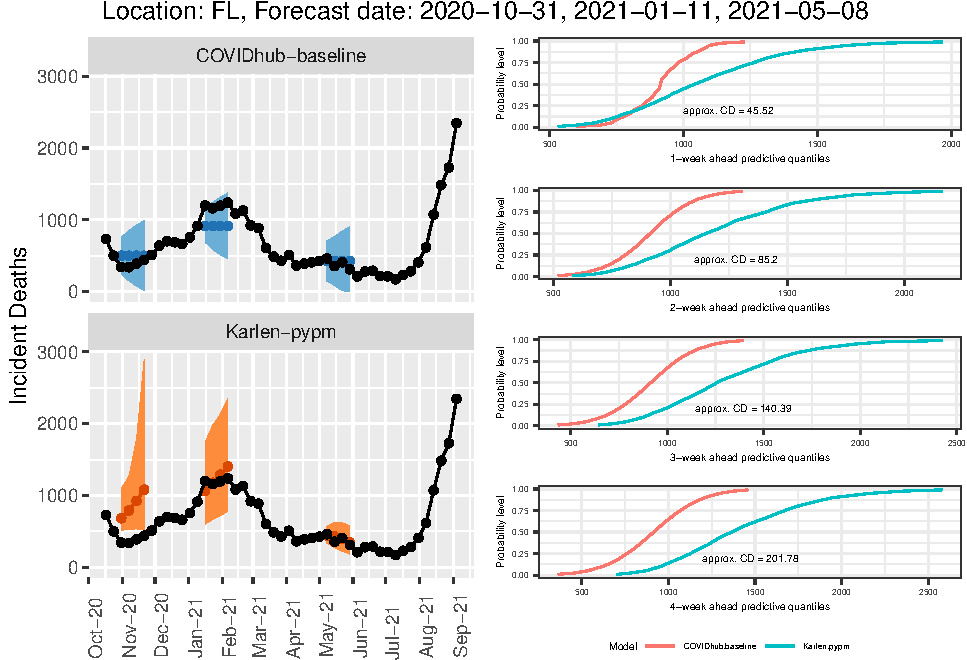
\includegraphics[width=0.8\linewidth,height=0.8\textheight]{cd_approx_2_files/figure-latex/unnamed-chunk-4-1} \end{center}

\begin{center}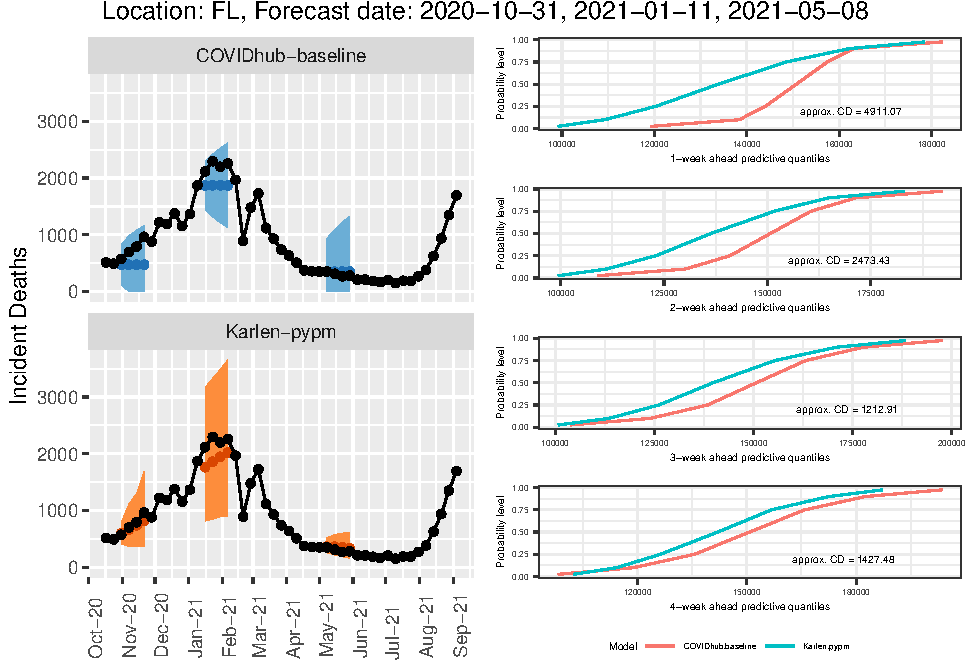
\includegraphics[width=0.8\linewidth,height=0.8\textheight]{cd_approx_2_files/figure-latex/unnamed-chunk-5-1} \end{center}

\hypertarget{similarity-focusing-on-the-beginnings-and-peaks-of-covid-waves}{%
\subsection{Similarity (focusing on the beginnings and peaks of COVID
waves)}\label{similarity-focusing-on-the-beginnings-and-peaks-of-covid-waves}}

\begin{center}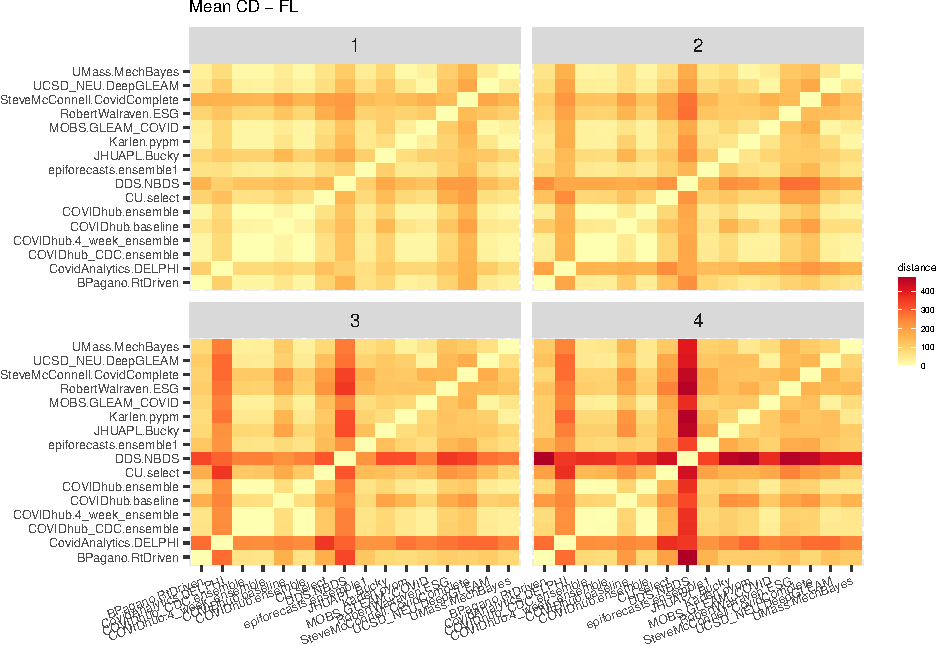
\includegraphics{cd_approx_2_files/figure-latex/unnamed-chunk-6-1} 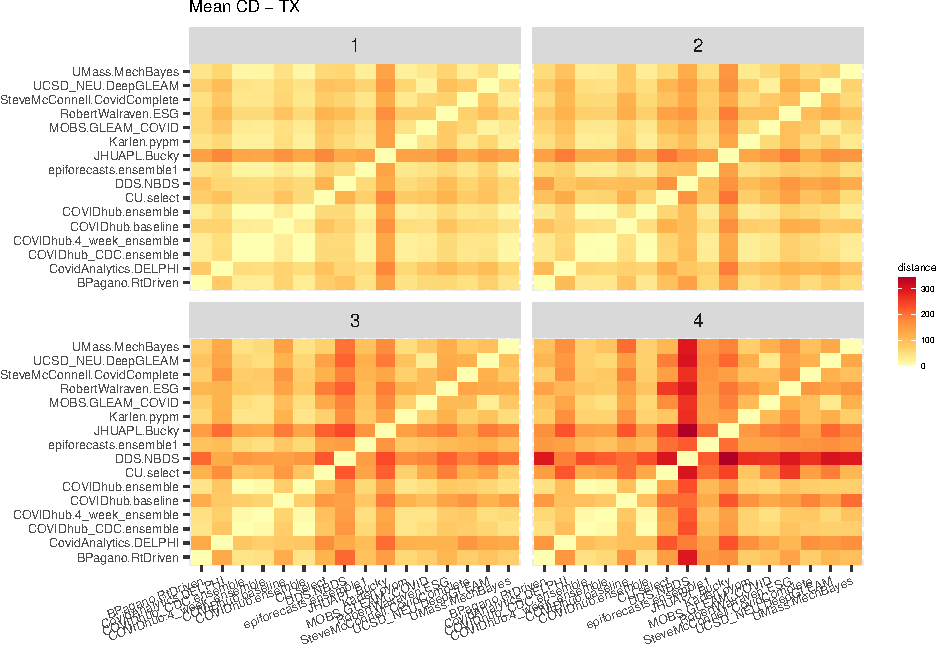
\includegraphics{cd_approx_2_files/figure-latex/unnamed-chunk-6-2} \end{center}

\begin{center}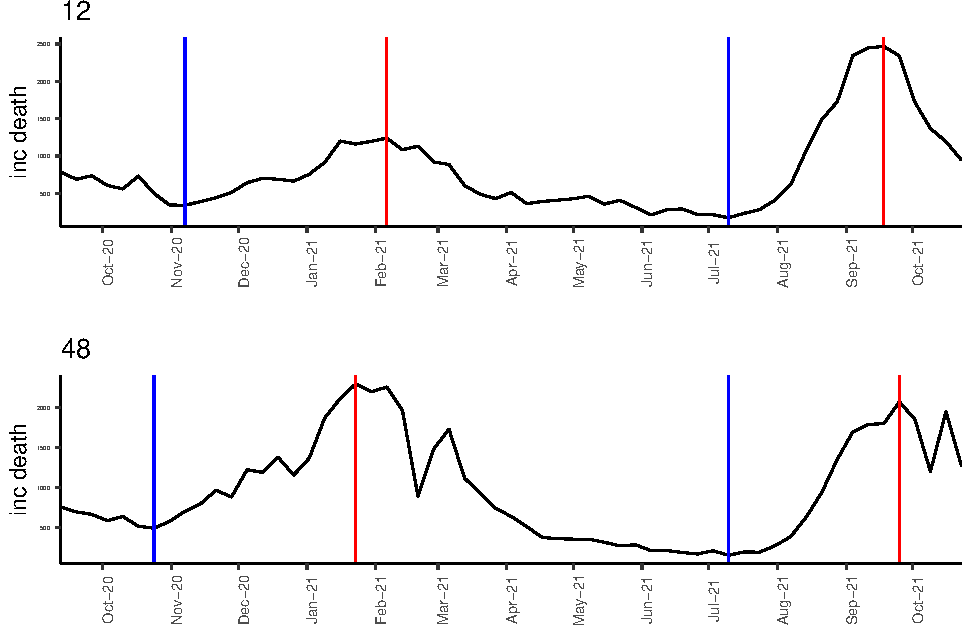
\includegraphics{cd_approx_2_files/figure-latex/unnamed-chunk-7-1} \end{center}

\begin{center}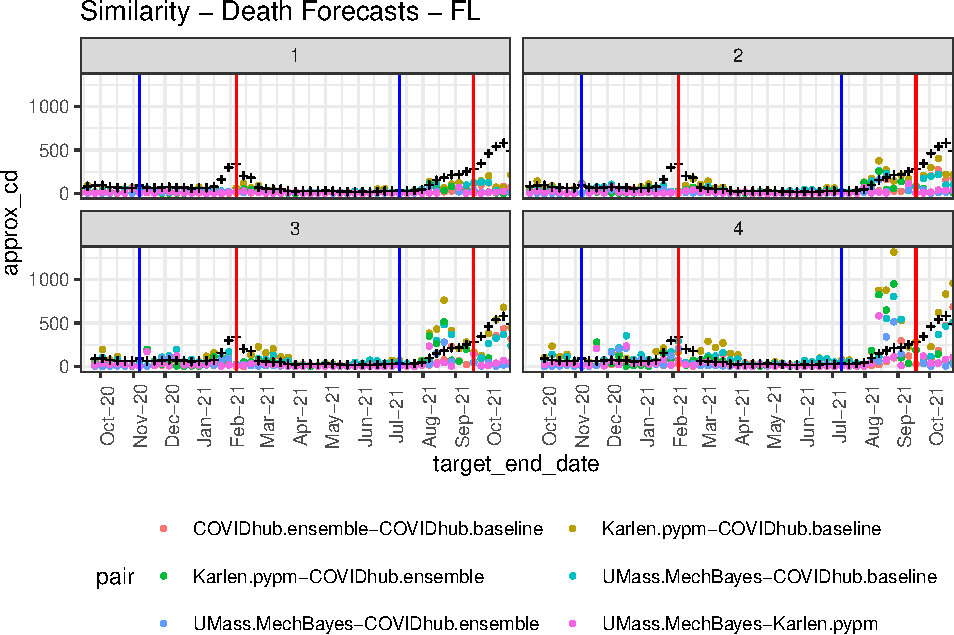
\includegraphics{cd_approx_2_files/figure-latex/unnamed-chunk-8-1} \end{center}

Combine all lead time into one?

\begin{center}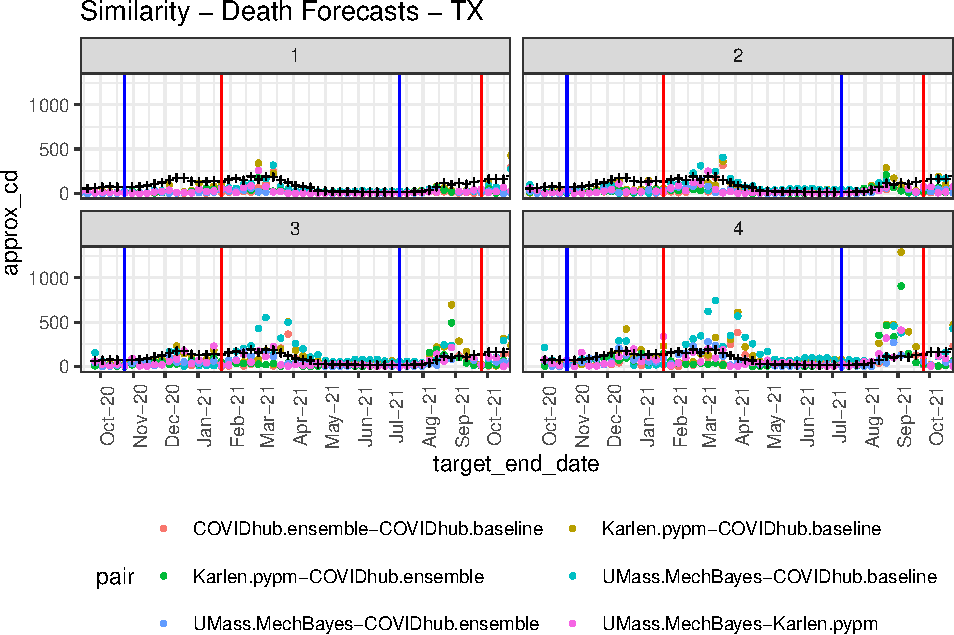
\includegraphics{cd_approx_2_files/figure-latex/unnamed-chunk-9-1} \end{center}

\hypertarget{correlation-between-wis-and-sd-of-approx.-cd}{%
\subsection{Correlation between WIS and SD of Approx.
CD}\label{correlation-between-wis-and-sd-of-approx.-cd}}

Assumption is that higher SD is correlated with worse WIS.
Predictability?

\hypertarget{consistencystability-of-models-and-ensemble}{%
\subsection{Consistency/stability of models and
ensemble}\label{consistencystability-of-models-and-ensemble}}

\hypertarget{approximating-the-cramer-distance-using-interval-divergences}{%
\subsection{Approximating the Cramer distance using interval
divergences}\label{approximating-the-cramer-distance-using-interval-divergences}}

Assuming \(K\) is even, the \(K\) equally spaced predictive quantiles of
each distribution can seen as \(L = K/2\) central prediction intervals
with coverage levels \(\alpha_i = 2i/(L + 1), i = 1, \dots, L\).
Similarly to the definition of the WIS, the approximation
\eqref{eq:approx_cd} can also be expressed in terms of these intervals
as

\[
\text{CD}(F, G) \approx \frac{1}{2L(2L + 1)}\sum_{k = 1}^L\sum_{m = 1}^L \text{ID}([l^F_k, u^F_k], [l^G_m, u^G_m], \alpha_k^F, \alpha_m^G).
\] This implies a decomposition of the Cramer distance into the four
interpretable components defined for the interval divergence in the
previous section. If \(G\) is a one-point distribution, the CD reduces
to the WIS and the proposed decomposition reduces to the well-known
decomposition of the WIS into dispersion, overprediction and
underprediction components.

Note that in practice we usually have an uneven rather than even number
\(K\) of predictive quantiles. In this case the median needs to be
treated separately (comparisons of the ``0\% prediction interval'\,'
need to be weighted down with a factor of 2; this is the same little
quirk as the one identified by Ryan and Evan for the WIS a few months
ago). The decomposition has the following properties:

\begin{itemize}
\item Additive shifts of the two distributions only affect the shift components, not the dispersion components.
\item Consequently, if $G$ and $G$ are identical up to an additive shift, both dispersion components will be 0.
\item If $F$ and $G$ are both symmetric and have the same median, the both shift components will be 0.
\item I think that in general it is possible that both shift components or both dispersion components are greater than 0, which leads to a somewhat strange interpretation. But this should only concern constructed examples.
\end{itemize}

\hypertarget{decomposition-preliminaries}{%
\subsection{Decomposition
Preliminaries}\label{decomposition-preliminaries}}

\hypertarget{motivation-of-the-approximation}{%
\subsubsection{Motivation of the
approximation}\label{motivation-of-the-approximation}}

We start by splitting up the sum from \eqref{eq:approx_cd} into
\begin{align}
\text{CD}(F, G) & \approx \frac{1}{K(K + 1)}\sum_{i = 1}^K\sum_{j = 1}^K 2 \times \mathbf{1}\{i \leq j \land q^F_i > q^G_j\} \times \left( q^F_i - q^G_j\right) \label{eq:two_sums} \\
& \ \ \ \ + \ \ \ \frac{1}{K(K + 1)}\sum_{i = 1}^K\sum_{j = 1}^K 2 \times \mathbf{1}\{i \geq j \land q^F_i < q^G_j\} \times \left( q^G_j - q^F_i\right) \nonumber
\end{align} We now denote by \(q_1 \leq q_2 \leq \dots \leq q_{2n}\) the
pooled set of quantiles (across \(F\) and \(G\)). Further, we denote by
\(r^F_1, \dots r^F_n\) and \(r^G_1, \dots r^G_n\) the ranks of the
members of \(q^F_1, \dots, q^F_n\) and \(q^G_1, \dots, q^G_n\),
respectively, within the pooled set of quantiles, i.e. \begin{equation}
q^F_i = q_{r^F_i}.\label{eq:substitution}
\end{equation} Note that ranks are oriented such that larger ranks
correspond to larger values. We now focus on the first of the two double
sums from equation \eqref{eq:two_sums}, which using
\eqref{eq:substitution} becomes \begin{align}
% & \frac{1}{K(K + 1)}\sum_{i = 1}^K\sum_{j = 1}^K 2 \times \mathbf{1}\{i \leq j \land q^F_i > q^G_j\} \times \left( q^F_i - q^G_j\right) \\
\frac{1}{K(K + 1)}\sum_{i = 1}^K\sum_{j = 1}^K 2 \times \mathbf{1}\{i \leq j \land r^F_i > r^G_j\} \times \left( q_{r^F_i} - q_{r^G_j}\right). \label{eq:to_continue}
\end{align} Now denote by \[
\delta_l = q_{l + 1} - q_l
\] the increments in the pooled set of quantiles. We can then use a
telescope sum and continue \eqref{eq:to_continue} as \begin{align}
% & \frac{1}{K(K + 1)}\sum_{i = 1}^K\sum_{j = 1}^K 2 \times \mathbf{1}\{i \leq j \land r^F_i > r^G_j\} \times \left( q_{r^F_i} - q_{r^G_j}\right)\\
= & \frac{1}{K(K + 1)}\sum_{i = 1}^K\sum_{j = 1}^K 2 \times \mathbf{1}\{i \leq j \land r^F_i > r^G_j\} \times \sum_{l = r^G_j}^{r^F_{i - 1}} \delta_l\\
= & \frac{1}{K(K + 1)} \sum_{l = 1}^{K} \delta_l \times 2 \times \sum_{i = 1}^K\sum_{j = 1}^K \mathbf{1}\{i \leq j \land r^G_j \leq l < r^F_i\}. \label{eq:second_sum2}\\
\end{align} The double sum over the indicator function counts how many
pairs of \((i, j)\) exist for a given \(l\) such that \(r^F_i\), but not
\(r^G_j\) exceeds \(l\), despite \(i \leq j\). To determine this number
consider \begin{align}
a^F_l & = \sum_{i = 1}^n \mathbf{1}(r^F_i \leq l)\\
a^G_l & = \sum_{i = 1}^n \mathbf{1}(r^G_i \leq l),
\end{align} i.e., the numbers of ranks falling below \(l\) among the
quantiles of \(F\) and \(G\). If \[
a_l^F - a_l^G = b_l \Leftrightarrow a_l^G = a_l^F - b_l
\] we have \begin{align}
r^F_{1} \leq \dots \leq r^F_{a_l^F} \leq l <  r^F_{a_l^F + 1} \leq \dots \leq r^F_n,\\
r^G_{1} \leq \dots \leq r^G_{a_l^F - b_l} \leq l <  r^F_{a_l^F - b_l + 1} \leq \dots \leq r^G_n.
\end{align} The case \((i \leq j \land r^G_j \leq l < r^F_i)\) thus
arises for

\begin{itemize}
\item[1.] the tuples $(r^F_{a^F_l}, r^G_{a^F_l}), (r^F_{a^F_l}, r^G_{a^F_l - 1}), \dots, (r^F_{a^F_l}, r^G_{a^F_l - (b_l - 1)})$, i.e. $b_l$ times for $r^F_{a^F_l}$.
\item[2.] the tuples $(r^F_{a^F_l - 1}, r^G_{a^F_l - 1}), (r^F_{a^F_l}, r^G_{a^F_l - 1}), \dots, (r^F_{a^F_l}, r^G_{a^F_l - (b_l - 1)})$, i.e. $b_l - 1$ times for $r^F_{a^F_l - 1}$.
\item[$\vdots$]
\item[$b_l$.] the tuple $(r^F_{a^F_l - b_l}, r^G_{a^F_l - b_l})$, i.e. once for $r^F_{a^F_l - b_l}$.
\end{itemize}

This results in a total of
\(b_l + (b_l -1) + \dots + 1 = b_l(b_l + 1)/2\) tuples, and we can
re-write expression \eqref{eq:second_sum2} as \[
= \frac{1}{K(K + 1)} \sum_{l = 1}^{K} \delta_l \times b_l(b_l + 1) \times \mathbf{1}(b_l > 0).
\] The same argument can be made for the second double sum in
\eqref{eq:two_sums}, and bringing the two back together again the
overall approximation from \eqref{eq:two_sums} simplifies to
\begin{equation}
\text{CD}(F, G) \approx \frac{1}{K(K + 1)} \sum_{l = 1}^{K} \delta_l \times b_l(b_l + 1). \label{eq:rectangles}
\end{equation} For large \(K\) we obviously have \begin{equation}
F(q_l) - G(q_l) = \underbrace{\frac{a^F_l}{K} - \frac{a^G_l}{K}}_{= b_l/K} \approx \underbrace{\frac{a^F_l + 1}{K + 1} - \frac{a^G_l + 1}{K + 1}}_{(b_l + 1)/(K + 1)}, \label{eq:approx_CDF}
\end{equation} meaning that \eqref{eq:rectangles} is a simple
(left-sided) Riemann sum approximation of the Cramer divergence.

There are more direct ways of approximating the Cramer divergence using
quantiles, e.g., using \(b_l^2\) rather than \(b_l \times (b_l + 1)\) in
\eqref{eq:rectangles}). The motivation for expression
\eqref{eq:approx_cd} is that if \(G\) is a point mass, the approximated
Cramer divergence simplifies to the approximation
\eqref{eq:linear_quantile_scores} already in use for the CRPS in the
context of forecast evaluation. To see this consider equation
\eqref{eq:two_sums}. With \(q^G_1 = \dots = q^G_K = y\) it becomes
\begin{align*}
\text{CD}(F, G) & \approx \frac{1}{K(K + 1)}\sum_{i = 1}^K\sum_{j = 1}^K 2\times \mathbf{1}(i \leq j \land q^F_i > y) \times \left( q^F_i - y\right) \\
& \ \ \ \ + \ \ \ \frac{1}{K(K + 1)}\sum_{i = 1}^K\sum_{j = 1}^K 2 \times \mathbf{1}(i \geq j \land q^F_i < y) \times \left(y - q^F_i\right)\\
& = \frac{1}{K(K + 1)} \left\{\sum_{i = 1}^K 2\times \mathbf{1}(q^F_i > y) \times i \times \left( q^F_i - y\right) \ \ + \ \ \sum_{i = 1}^K 2 \times \mathbf{1}(q^F_i < y) \times (K + 1 - i) \times \left(y - q^F_i\right)\right\}\\
& = \frac{1}{K(K + 1)} \sum_{i = 1}^K 2\times \{\mathbf{1}(q^F_i > y) \times (K + 1) - i\} \times (q^F_i - y) \\
& = \frac{1}{K} \sum_{i = 1}^K 2\times \{\mathbf{1}(q^F_i > y) - i/(K + 1)\} \times (q^F_i - y).
\end{align*} This is precisely the approximation of the CRPS from
equation \eqref{eq:linear_quantile_scores}.

\hypertarget{establishing-a-decomposition-for-the-approximated-cramer-distance}{%
\subsection{Establishing a decomposition for the approximated Cramer
distance}\label{establishing-a-decomposition-for-the-approximated-cramer-distance}}

We now introduce a decomposition of the approximated Cramer distance
into the four following components:

\begin{itemize}
\item larger dispersion of $F$ relative to $G$,
\item larger dispersion of $G$ relative to $F$,
\item upward shift of $F$ relative to $G$,
\item upward shift of $G$ relative to $F$.
\end{itemize}

This decomposition is inspired by the decomposition of the interval
score which translates to the weighted interval score (WIS). To extend
it to the approximated Cramer distance, we need to express it in terms
of symmetric prediction intervals, similar to the definition of the WIS
via the interval score. In the following we introduce such a
representation and decomposition.

\hypertarget{a-divergence-measure-for-central-prediction-intervals-with-potentially-different-nominal-coverages}{%
\subsubsection{A divergence measure for central prediction intervals
with potentially different nominal
coverages}\label{a-divergence-measure-for-central-prediction-intervals-with-potentially-different-nominal-coverages}}

Consider two central prediction intervals \([l^F, u^F]\) and
\([l^G, u^G]\) with nominal levels \(\alpha^F, \alpha^G \in [0, 1)\),
respectively; \(l^F\) is thus the \((1 - \alpha^F)/2\) quantile of
\(F\), \(u^F\) is the \((1 + \alpha^F)/2\) quantile of \(F\) etc. Note
that we include the boundary case \(\alpha = 0\), even though it has
somewhat peculiar behaviour. We can define an
\textit{interval divergence} measure by comparing the two pairs of
predictive quantiles and summing up the four resulting incompatibility
penalties as in \eqref{eq:approx_cd}. Writing this out completely gives
the somewhat unwieldy expression \begin{align*}
\text{ID}([l^F, u^F], [l^G, u^G], \alpha^F, \alpha^G) = & \ \ \ \mathbf{1}\big\{\{(1 - \alpha^F)/2 \leq (1 - \alpha^G)/2 \land l^F > l^G\big\} \\
& \ \ \ \ \ \ \ \ \ \ \ \ \ \ \lor \{(1 - \alpha^F)/2 \geq (1 - \alpha^G)/2 \land l^F < l^G\}\} \times |l^F - l^G|\\
& \ \ \ \ \ \ \ \ \ \ + \ \mathbf{1}\big\{\{(1 - \alpha^F)/2 \leq (1 + \alpha^G)/2 \land l^F > u^G\big\} \\
& \ \ \ \ \ \ \ \ \ \ \ \ \ \ \ \ \ \ \ \lor \{(1 - \alpha^F)/2 \geq (1 + \alpha^G)/2 \land l^F < u^G\}\} \times |l^F - u^G|\\
& \ \ \ \ \ \ \ \ \ \ + \ \mathbf{1}\big\{\{(1 + \alpha^F)/2 \leq (1 - \alpha^G)/2 \land u^F > l^G\big\} \\
& \ \ \ \ \ \ \ \ \ \ \ \ \ \ \ \ \ \ \ \lor \{(1 + \alpha^F)/2 \geq (1 - \alpha^G)/2 \land u^F < l^G\}\} \times |u^F - l^G|\\
& \ \ \ \ \ \ \ \ \ \ + \ \mathbf{1}\big\{\{(1 + \alpha^F)/2 \leq (1 + \alpha^G)/2 \land u^F > u^G\big\} \\
& \ \ \ \ \ \ \ \ \ \ \ \ \ \ \ \ \ \ \ \lor \{(1 + \alpha^F)/2 \geq (1 + \alpha^G)/2 \land u^F < u^G\}\} \times |u^F - u^G|.
\end{align*} By construction we know that if \(\alpha^F > 0\) or
\(\alpha^G > 0\) we have \(1 - \alpha^F < 1 + \alpha^G\) and
\(1 - \alpha^G < 1 + \alpha^F\) while
\((1 - \alpha^F)/2 \leq (1 - \alpha^G)/2 \Leftrightarrow \alpha_F \geq \alpha^G \Leftrightarrow (1 + \alpha^F)/2 \geq (1 + \alpha^G)/2\)
etc. In this case the above can thus be simplified considerably to
\begin{align*}
\text{ID}([l^F, u^F], [l^G, u^G], \alpha^F, \alpha^G) = & \ \mathbf{1}(\alpha^F \leq \alpha^G)\times\left\{\max(l^G - l^F, 0) + \max(u^F - u^G, 0)\right\} \\
& \ \ \ \ \ \ \ \ + \ \mathbf{1}(\alpha^F \geq \alpha^G) \times \left\{\max(l^F - l^G, 0) + \max(u^G - u^F, 0)\right\} \\
& \ \ \ \ \ \ \ \ + \max(l^F - u^G, 0) \ +\\
& \ \ \ \ \ \ \ \ + \max(l^G - u^F, 0).
\end{align*}

Here, the first row adds penalties for the case where \([l^F, u^F]\)
should be nested in \([l^G, u^G]\), but at least one of its ends is more
extreme than the respective end of \([l^G, u^G]\). The second row covers
the converse case. The last two rows add penalties if the lower end of
one interval exceeds the upper end of the other, i.e.~the intervals do
not overlap. This can be seen as a (scaled version of a) generalization
of the interval score, but writing out the exact relationship is a bit
tedious.

If \(\alpha^F = \alpha^G = 0\) we have \[
\text{ID}([l^F, u^F], [l^G, u^G], 0, 0) = 4 \times |m^F - m^G|
\] where \(m^F = l^F = u^F\) and \(m^G = l^G = u^G\) are the predictive
medians of \(F\) and \(G\), respectively.

We now define four auxiliary terms with an intuitive interpretation
which add up to the interval divergence:

\begin{itemize}
\item The term
$$
D_F = \mathbf{1}(\alpha^F \leq \alpha^G)\times\max\{(u^F - l^F) - (u^G - l^G), 0\}
$$
is the sum of penalties resulting from $F$ being more dispersed than $G$. It is positive whenever the interval $[l^F, u^F]$ is longer than $[l^G, u^G]$, even though it should be nested in the latter. $D_F$ then tells us by how much we would need to shorten $[l^F, u^F]$ so it could fit into $[l^G, u^G]$.
\item The term
$$
D_G = \mathbf{1}(\alpha^G \leq \alpha^G)\times\max\{(u^G - l^G) - (u^F - l^F), 0\}
$$
measures the converse, i.e. overdispersion of $G$ relative to $F$. Note that at most one of $D_F$ and $D_G$ can be positive. If $\alpha^F = \alpha^G = 0$ we always have $D^F = D^G = 0$.
\item The term
$$
S^F = \mathbf{1}\left\{l^F + u^F > l^G + u^G \right\} \times \left\{\text{ID}([l^F, u^F], [l^G, u^G], \alpha^F, \alpha^G) - D^F - D^G\right\}
$$
% $$
% S^F = \max\{\mathbf{1}(\alpha^G \leq \alpha^F) \times \max(l^F - l^G, 0) + \mathbf{1}(\alpha^F \leq \alpha^G) \times \max(u^F - u^G, 0) + \max(l^F - u^G, 0) - D_F - D_G, 0\}
% $$
represents an \textit{upward shift} of $F$ relative to $G$. It is zero unless the center of $[l^F + u^F]$ exceeds that of $[l^G + u^G]$, in which case it absorbs the remaining penalties after accounting for differences in dispersion via $D^F$ and $D^G$.
\item The term
$$
S^G = \mathbf{1}\left\{l^F + u^F < l^G + u^G\right\} \times \left\{\text{ID}([l^F, u^F], [l^G, u^G], \alpha^F, \alpha^G) - D^F - D^G\right\}
$$
% $$
% S^G = \max\{\mathbf{1}(\alpha^F \leq \alpha^G) \times \max(l^G - l^F, 0) + \mathbf{1}(\alpha^G \leq \alpha^F) \times \max(u^G - u^F, 0) + \max(l^G - u^F, 0) - D_G - D_F, 0\}
% $$
accordingly represents an \textit{upward shift} of $G$ relative to $F$. Again note that at most one out of $S^F$ and $S^G$ can be positive.
\end{itemize}

It is easy to see that \[
\text{ID}([l^F, u^F], [l^G, u^G], \alpha^F, \alpha^G) = D^F + D^G + S^F + S^G.
\] Intuitively the interval divergence measures by how much we need to
move the quantiles of the interval with lower nominal coverage so it
fits into the one with larger nominal coverage. The different components
correspond to different types of moves we can make to achieve this We
illustrate this using an example: Assume \([l^F, u^F]\) has lower
nominal coverage than \([l^G, u^G]\), but is wider while \(l^F > u^G\)
(i.e.,~the intervals are non-overlapping):

\bigskip

\begin{tikzpicture}[x=1cm,y=0.28cm]
\draw[-] (1, 1) -- (4, 1);
\draw[-] (1, 0.7) -- (1, 1.3);
\draw[black,fill=white](1,0) node {$l^G$};
\draw[-] (4, 0.7) -- (4, 1.3);
\draw[black,fill=white](4,0) node {$u^G$};

\draw[-] (5, 4) -- (11, 4);
\draw[-] (5, 3.7) -- (5, 4.3);
\draw[black,fill=white](5,3) node {$l^F$};
\draw[-] (11, 3.7) -- (11, 4.3);
\draw[black,fill=white](11,3) node {$u^F$};
\end{tikzpicture}

To fit \([l^F, u^F]\) into \([l^G, u^G]\) we first need to shorten it by
\(D^F = (u^F - l^F) - (u^G - l^G)\). We perform this shortening at the
end which is furthest from \([l^G, u^G]\):

\begin{tikzpicture}[x=1cm,y=0.28cm]
\draw[-] (1, 1) -- (4, 1);
\draw[-] (1, 0.7) -- (1, 1.3);
\draw[black,fill=white](1,0) node {$l^G$};
\draw[-] (4, 0.7) -- (4, 1.3);
\draw[black,fill=white](4,0) node {$u^G$};

\draw[-, dotted] (5, 4) -- (11, 4);
\draw[-] (5, 4) -- (8, 4);
\draw[-] (5, 3.7) -- (5, 4.3);
\draw[-] (8, 3.7) -- (8, 4.3);
\draw[black,fill=white](5,3) node {$l^F$};
\draw[-] (11, 3.7) -- (11, 4.3);
\draw[black,fill=white](11,3) node {$u^F$};

\draw[->] (11, 4.0) arc (-155:-35:-1.7) ;

\end{tikzpicture}

Then we shift both ends of the resulting interval just onto the upper
end \(u^G\) of the interval with larger nominal coverage:

\begin{tikzpicture}[x=1cm,y=0.28cm]
\draw[-] (1, 1) -- (4, 1);
\draw[-] (1, 0.7) -- (1, 1.3);
\draw[black,fill=white](1,0) node {$l^G$};
\draw[-] (4, 0.7) -- (4, 1.3);
\draw[black,fill=white](4,0) node {$u^G$};

\draw[-, dotted] (5, 4) -- (8, 4);
\draw[-] (5, 3.7) -- (5, 4.3);
\draw[-] (8, 3.7) -- (8, 4.3);
\draw[black,fill=white](5,3) node {$l^F$};

\draw[->] (8, 4.0) arc (-155:-35:-2.3) ;
\draw[->] (5, 4.0) arc (-155:-35:-.55) ;

\draw[-] (4, 3.7) -- (4, 4.3);

\end{tikzpicture}

The sum of the two necessary shifts (of the upper and lower end), which
in this case simplifies to \(S^F = 2l^F - u^G -l^G\) can be interpreted
as the upward shift of \([l^F, u^F]\) with respect to \(l^G, u^G]\).

\hypertarget{approximating-the-cramer-distance-using-interval-divergences-1}{%
\subsubsection{Approximating the Cramer distance using interval
divergences}\label{approximating-the-cramer-distance-using-interval-divergences-1}}

Assuming \(K\) is even, the \(K\) equally spaced predictive quantiles of
each distribution can seen as \(L = K/2\) central prediction intervals
with coverage levels \(\alpha_i = 2i/(L + 1), i = 1, \dots, L\).
Similarly to the definition of the WIS, the approximation
\eqref{eq:approx_cd} can also be expressed in terms of these intervals
as \[
\text{CD}(F, G) \approx \frac{1}{2L(2L + 1)}\sum_{k = 1}^L\sum_{m = 1}^L 2 \times \text{ID}([l^F_k, u^F_k], [l^G_m, u^G_m], \alpha_k^F, \alpha_m^G).
\] This is easily seen as the involved double sum runs over the same
discrepancy penalties as the one in equation \eqref{eq:approx_cd}, with
four of them covered in each of the computed interval divergences.

If \(K\) is uneven, we get \(L = (2K + 1)/2\) central prediction
intervals for each distribution, with coverage levels
\(\alpha_i = 2(i - 1)/(L + 1), i = 1, \dots, L\). This means that the
innermost prediction interval is just a single point at the predictive
median. To avoid penalizing incompatibilities involving one of the
medians more than once we then need to adjust the above to
\begin{equation}
\text{CD}(F, G) \approx \frac{1}{(2L - 0.5)(2L + 0.5)}\sum_{k = 1}^L\sum_{m = 1}^L w_{km}\text{ID}([l^F_k, u^F_k], [l^G_m, u^G_m], \alpha_k^F, \alpha_m^G).
\end{equation} with \[
w_{km} = \begin{cases} 1/4 & \text{ if } k = 0 = m \\
1/2 & \text{ if } k = 0 \neq m \text{ or } k = 0 \neq m\\
1 & \text{else}
\end{cases}.
\]

This representation implies a decomposition of the Cramer distance into
the four interpretable components defined for the interval divergence in
the previous section. Each component is just defined as the
(appropriately weighted) average of the respective components at the
different coverage levels. If \(G\) is a one-point distribution, the CD
reduces to the WIS and the proposed decomposition reduces to the
well-known decomposition of the WIS into dispersion, overprediction and
underprediction components. The decomposition has the following further
properties:

\begin{itemize}
\item Additive shifts of the two distributions affect the shift components, but not the dispersion components.
\item Consequently, if $G$ and $G$ are identical up to an additive shift, both dispersion components will be 0.
\item If $F$ and $G$ are both symmetric and have the same median, both shift components will be 0.
\item It is possible that both shift components or both dispersion components are greater than 0, which leads to a somewhat strange interpretation. This corresponds to CDFs which cross more than once.
\end{itemize}

\hypertarget{examples}{%
\section{Examples}\label{examples}}

\hypertarget{equally-spaced-intervals}{%
\subsection{Equally-spaced intervals}\label{equally-spaced-intervals}}

\begin{center}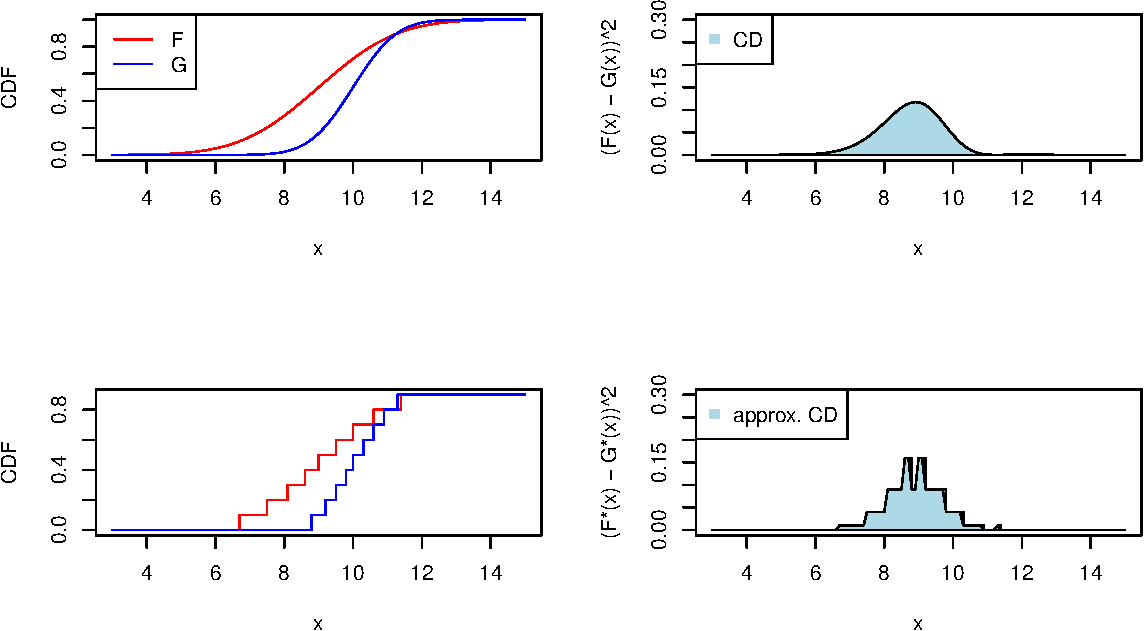
\includegraphics{cd_approx_2_files/figure-latex/unnamed-chunk-11-1} \end{center}

In this example, six different approximations are applied to the
distributions \(F~N(9, 1.8)\) and \(G~N(10, 1)\) in the figures above.

\begin{itemize}
\tightlist
\item
  Using direct numerical integration based on a fine grid of values for
  \(x\):
\end{itemize}

\begin{verbatim}
FALSE [1] 0.2532376
\end{verbatim}

\begin{itemize}
\tightlist
\item
  Using sampling and the alternative expression
  \eqref{eq:formulation_expectations} of the CD from above:
\end{itemize}

\begin{verbatim}
FALSE [1] 0.2457156
\end{verbatim}

\begin{itemize}
\tightlist
\item
  Using the first quantile-based approximation \eqref{eq:approx2} and
  various values of \(K\):
\end{itemize}

\begin{verbatim}
FALSE [1] 0.3550788 0.3078906 0.2764153 0.2652018 0.2593619 0.2557450 0.2545077
FALSE [8] 0.2538792
\end{verbatim}

\begin{itemize}
\tightlist
\item
  Using the second quantile-based approximation \eqref{eq:approx2} and
  various values of \(K\):
\end{itemize}

\begin{verbatim}
FALSE [1] 0.2926809 0.2723571 0.2608768 0.2572045 0.2552998 0.2541028 0.2536835
FALSE [8] 0.2534662
\end{verbatim}

\begin{itemize}
\tightlist
\item
  Using the left-sided Riemann sum approximation and various values of
  \(K\):
\end{itemize}

\begin{verbatim}
FALSE [1] 0.2370715 0.2458022 0.2505461 0.2520862 0.2527531 0.2530874 0.2531764
FALSE [8] 0.2532128
\end{verbatim}

\begin{itemize}
\tightlist
\item
  Using the trapezoidal Riemann sum approximation and various values of
  \(K\):
\end{itemize}

\begin{verbatim}
FALSE [1] 0.2854597 0.2575762 0.2543386 0.2552775 0.2540318 0.2535609 0.2534094
FALSE [8] 0.2533309
\end{verbatim}

The below plot shows the results from the different computations.

\begin{center}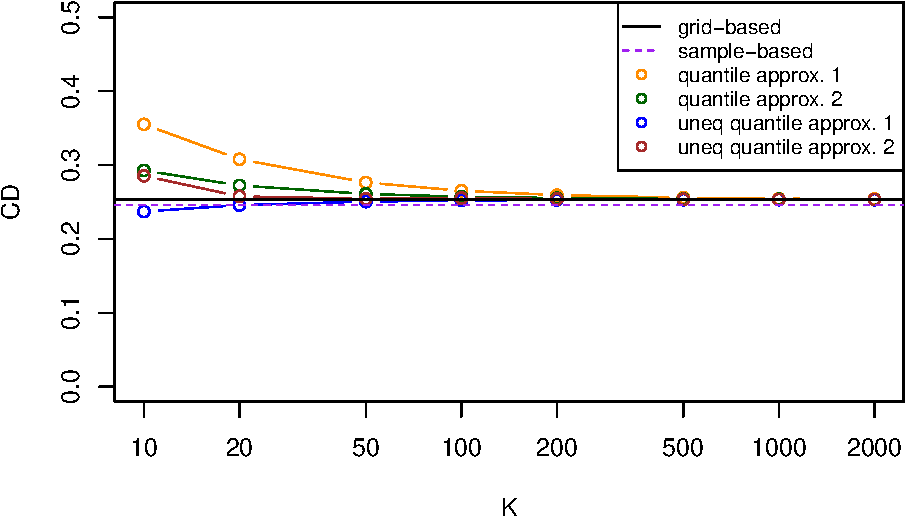
\includegraphics{cd_approx_2_files/figure-latex/unnamed-chunk-19-1} \end{center}

In the case that \(G\) is a point mass at \(y=10\), approximation
\eqref{eq:approx1} indeed coincides with
\eqref{eq:linear_quantile_scores}.

\begin{verbatim}
FALSE [1] "Quantile approx. 1: 0.688567227886639"
\end{verbatim}

\begin{verbatim}
FALSE [1] "Quantile approx. 2: 0.608983067073759"
\end{verbatim}

\begin{verbatim}
FALSE [1] "Uneq quantile approx. 1: 1.03814992169128"
\end{verbatim}

\begin{verbatim}
FALSE [1] "Uneq quantile approx. 2: 1.24791020451193"
\end{verbatim}

\begin{verbatim}
FALSE [1] "Quantile score WIS: 0.688567227886639"
\end{verbatim}

The approximation \eqref{eq:approx1} is closer to the grid-based direct
evaluation of the integral. Since the unequally-spaced approximations
were not formulated from (equally-spaced) WIS, it may be expected.

\begin{verbatim}
FALSE [1] "Grid-based approx.: 0.61599852942592"
\end{verbatim}

\hypertarget{unequally-spaceed-intervals}{%
\subsection{Unequally-spaceed
intervals}\label{unequally-spaceed-intervals}}

We apply the same six approximations as in the previous example to the
two distributions \(F\sim N(8,2)\) and \(G \sim N(11,1)\) whose
quantiles correspond to unequally-spaced probability levels.

\hypertarget{quantiles-with-unequally-spaced-intervals}{%
\subsubsection{7 quantiles with unequally-spaced
intervals}\label{quantiles-with-unequally-spaced-intervals}}

The probability levels corresponding to the given set of quantiles in
this example is \(0.025,0.1,0.25,0.5,0.75,0.9,0.975\), which is the same
probability levels provided by the COVID-hub case forecasts.

\begin{center}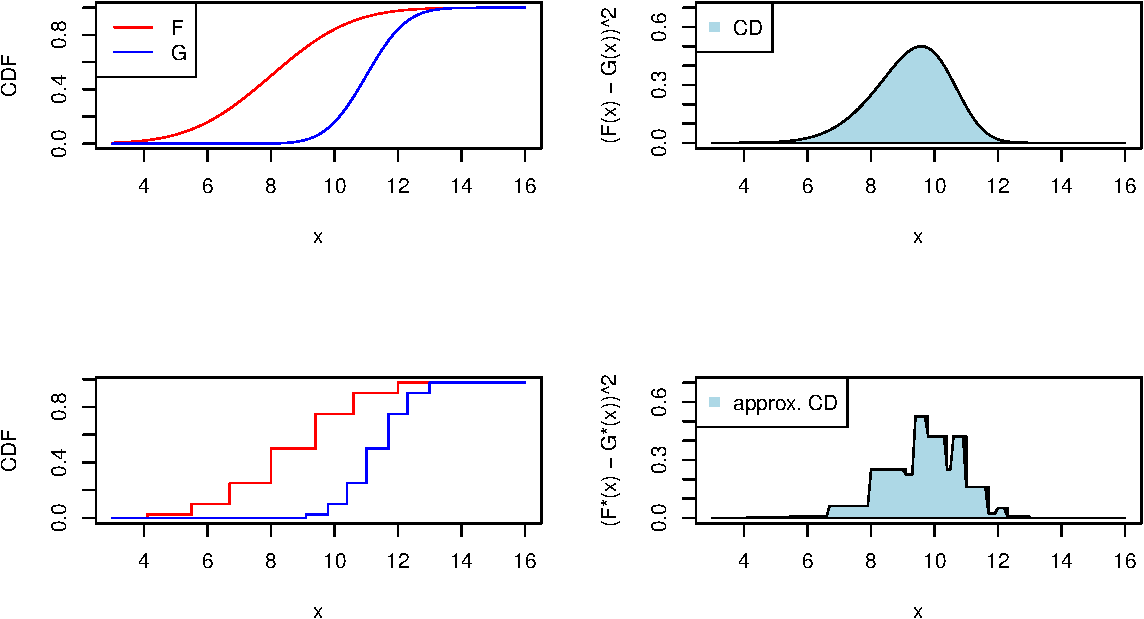
\includegraphics{cd_approx_2_files/figure-latex/unnamed-chunk-22-1} \end{center}

\begin{itemize}
\tightlist
\item
  Using direct numerical integration based on a fine grid of values for
  \(x\).
\end{itemize}

\begin{verbatim}
FALSE [1] 1.493653
\end{verbatim}

\begin{itemize}
\tightlist
\item
  Using sampling and the alternative expression
  \eqref{eq:formulation_expectations} of the CD from above:
\end{itemize}

\begin{verbatim}
FALSE [1] 1.483948
\end{verbatim}

\begin{itemize}
\tightlist
\item
  Using the first quantile-based approximation:
\end{itemize}

\begin{verbatim}
FALSE [1] 1.919252
\end{verbatim}

\begin{itemize}
\tightlist
\item
  Using the second quantile-based approximation:
\end{itemize}

\begin{verbatim}
FALSE [1] 1.764859
\end{verbatim}

\begin{itemize}
\tightlist
\item
  Using the left-sided Riemann sum-based approximation:
\end{itemize}

\begin{verbatim}
FALSE [1] 1.35122
\end{verbatim}

\begin{itemize}
\tightlist
\item
  Using the trapezoidal Riemann sum-based approximation:
\end{itemize}

\begin{verbatim}
FALSE [1] 1.468801
\end{verbatim}

Out of all four quantile-based approximation, the trapezoidal Riemann
sum-based approximation is closest to the grid-based integral
evaluation.

\hypertarget{quantiles-with-2-unequally-spaced-probability-levels-at-the-tails}{%
\subsubsection{23 quantiles with 2 unequally-spaced probability levels
at the
tails}\label{quantiles-with-2-unequally-spaced-probability-levels-at-the-tails}}

Using the same \(F\) and \(G\), the probability levels corresponding to
the given set of quantiles in this example is the same probability
levels provided by the COVID-hub death forecasts. They are almost
equally-spaced, except at the tails.

\begin{center}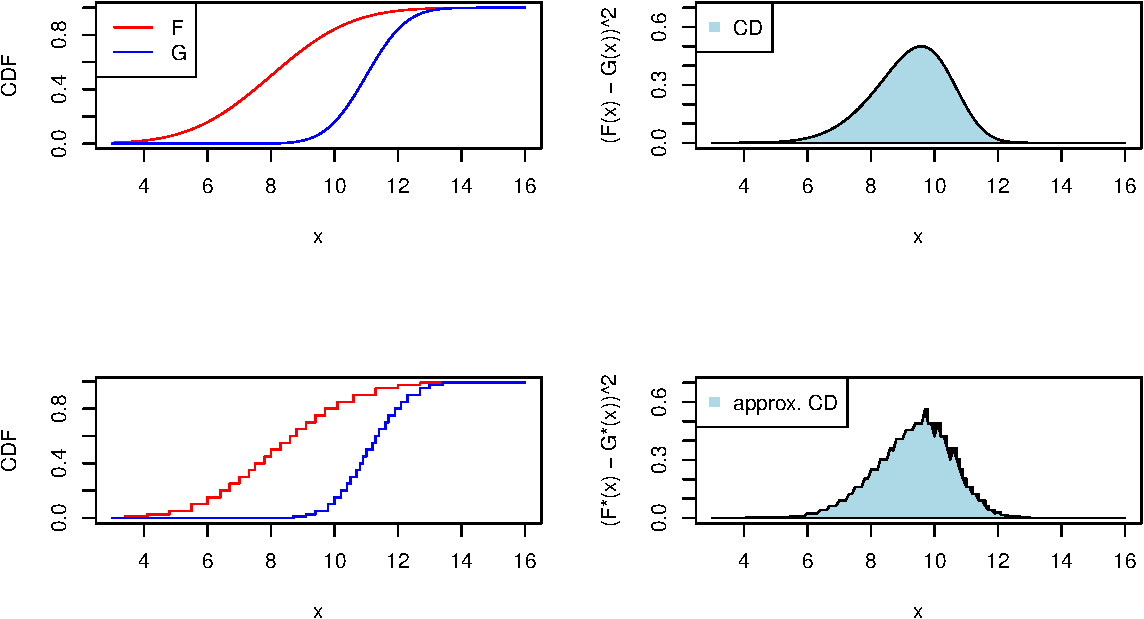
\includegraphics{cd_approx_2_files/figure-latex/unnamed-chunk-29-1} \end{center}

\begin{itemize}
\tightlist
\item
  Using the first quantile-based approximation:
\end{itemize}

\begin{verbatim}
FALSE [1] 1.640408
\end{verbatim}

\begin{itemize}
\tightlist
\item
  Using the second quantile-based approximation:
\end{itemize}

\begin{verbatim}
FALSE [1] 1.581296
\end{verbatim}

\begin{itemize}
\tightlist
\item
  Using the left-sided Riemann sum-based approximation:
\end{itemize}

\begin{verbatim}
FALSE [1] 1.452266
\end{verbatim}

\begin{itemize}
\tightlist
\item
  Using the trapezoidal Riemann sum-based approximation:
\end{itemize}

\begin{verbatim}
FALSE [1] 1.470718
\end{verbatim}

Again, the trapezoidal Riemann sum-based approximation is closest to the
grid-based integral evaluation of 1.493653.

\hypertarget{examples-of-disagreement-between-equally--and-unequally-spaced-interval-methods}{%
\subsubsection{Examples of Disagreement Between Equally- and
Unequally-spaced Interval
Methods}\label{examples-of-disagreement-between-equally--and-unequally-spaced-interval-methods}}

\hypertarget{heavy-tails}{%
\paragraph{Heavy tails}\label{heavy-tails}}

Suppose we have three cumulative distributions, \(F\sim N(1,1)\),
\(G\sim N(2,1)\) and \(H\sim T_1\), represented by 7 unequally-spaced
quantiles. The probability levels corresponding to the given set of
quantiles in this example is \(0.025,0.1,0.25,0.5,0.75,0.9,0.975\).

\begin{center}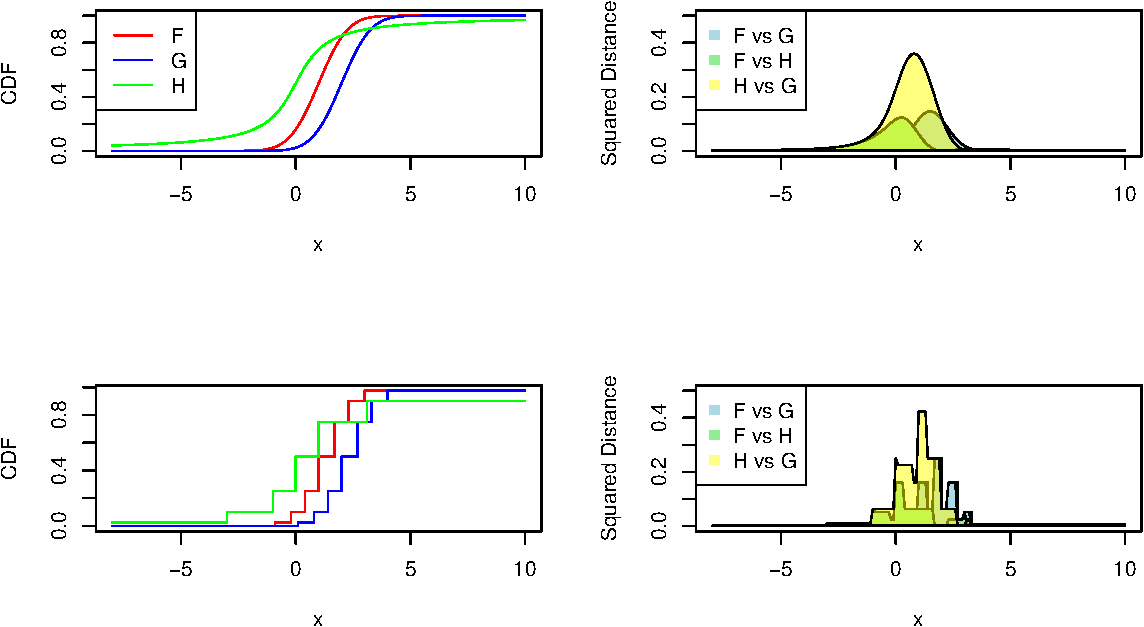
\includegraphics{cd_approx_2_files/figure-latex/unnamed-chunk-34-1} \end{center}

\begin{itemize}
\tightlist
\item
  Using direct numerical integration based on a fine grid of values for
  \(x\).
\end{itemize}

\begin{verbatim}
FALSE [1] "CD of F vs G: 0.270903289652979"
\end{verbatim}

\begin{verbatim}
FALSE [1] "CD of F vs H: 0.303008857878541"
\end{verbatim}

\begin{verbatim}
FALSE [1] "CD of H vs G: 0.830227986212452"
\end{verbatim}

\begin{itemize}
\tightlist
\item
  Using the first quantile-based approximation:
\end{itemize}

\begin{verbatim}
FALSE [1] "Approx. CD of F vs G: 0.430834455349389"
\end{verbatim}

\begin{verbatim}
FALSE [1] "Approx. CD of F vs H: 0.412836097817344"
\end{verbatim}

\begin{verbatim}
FALSE [1] " Approx. CD of H vs G: 1.0891147790307"
\end{verbatim}

\begin{itemize}
\tightlist
\item
  Using the second quantile-based approximation:
\end{itemize}

\begin{verbatim}
FALSE [1] "Approx. CD of F vs G: 0.349525091827873"
\end{verbatim}

\begin{verbatim}
FALSE [1] "Approx. CD of F vs H: 0.318185573750552"
\end{verbatim}

\begin{verbatim}
FALSE [1] " Approx. CD of H vs G: 0.958988318892232"
\end{verbatim}

\begin{itemize}
\tightlist
\item
  Using the left-sided Riemann sum-based approximation:
\end{itemize}

\begin{verbatim}
FALSE [1] "Approx. CD of F vs G: 0.267605148430715"
\end{verbatim}

\begin{verbatim}
FALSE [1] "Approx. CD of F vs H: 0.243610829902767"
\end{verbatim}

\begin{verbatim}
FALSE [1] " Approx. CD of H vs G: 0.734225431651865"
\end{verbatim}

\begin{itemize}
\tightlist
\item
  Using the trapezoidal Riemann sum-based approximation:
\end{itemize}

\begin{verbatim}
FALSE [1] "Approx. CD of F vs G: 0.302511061162121"
\end{verbatim}

\begin{verbatim}
FALSE [1] "Approx. CD of F vs H: 0.266926890705267"
\end{verbatim}

\begin{verbatim}
FALSE [1] " Approx. CD of H vs G: 0.752143988834321"
\end{verbatim}

\hypertarget{long-tails}{%
\paragraph{Long tails}\label{long-tails}}

Suppose we have three cumulative distributions, \(F\sim N(0,1)\),
\(G\sim N(1,1)\) and \(H\sim \text{Laplace}(0,1)\), represented by 7
unequally-spaced quantiles. The probability levels corresponding to the
given set of quantiles in this example is
\(0.025,0.1,0.25,0.5,0.75,0.9,0.975\).

\begin{center}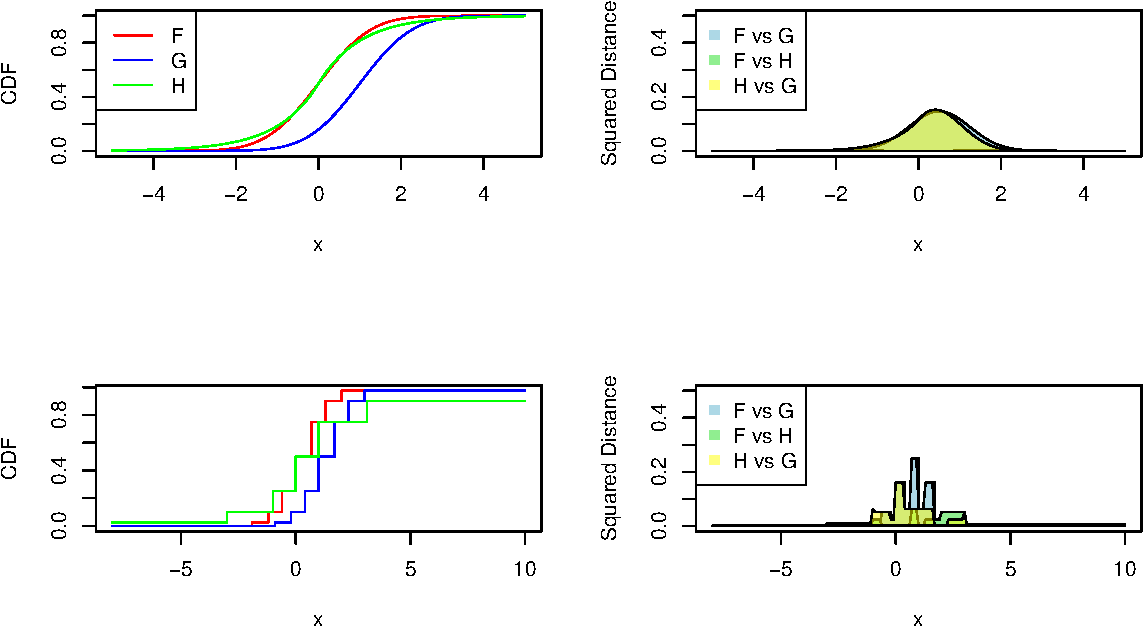
\includegraphics{cd_approx_2_files/figure-latex/unnamed-chunk-40-1} \end{center}

\begin{itemize}
\tightlist
\item
  Using direct numerical integration based on a fine grid of values for
  \(x\).
\end{itemize}

\begin{verbatim}
FALSE [1] "CD of F vs G: 0.270903289581517"
\end{verbatim}

\begin{verbatim}
FALSE [1] "CD of F vs H: 0.0068412250422997"
\end{verbatim}

\begin{verbatim}
FALSE [1] "CD of H vs G: 0.257655267503305"
\end{verbatim}

\begin{itemize}
\tightlist
\item
  Using the first quantile-based approximation:
\end{itemize}

\begin{verbatim}
FALSE [1] "Approx. CD of F vs G: 0.430834455349389"
\end{verbatim}

\begin{verbatim}
FALSE [1] "Approx. CD of F vs H: 0.0203971216157386"
\end{verbatim}

\begin{verbatim}
FALSE [1] " Approx. CD of H vs G: 0.416591384312851"
\end{verbatim}

\begin{itemize}
\tightlist
\item
  Using the second quantile-based approximation:
\end{itemize}

\begin{verbatim}
FALSE [1] "Approx. CD of F vs G: 0.349525091827873"
\end{verbatim}

\begin{verbatim}
FALSE [1] "Approx. CD of F vs H: 0.0116554980661363"
\end{verbatim}

\begin{verbatim}
FALSE [1] " Approx. CD of H vs G: 0.333247296357544"
\end{verbatim}

\begin{itemize}
\tightlist
\item
  Using the left-sided Riemann sum-based approximation:
\end{itemize}

\begin{verbatim}
FALSE [1] "Approx. CD of F vs G: 0.267605148430715"
\end{verbatim}

\begin{verbatim}
FALSE [1] "Approx. CD of F vs H: 0.00892374070688564"
\end{verbatim}

\begin{verbatim}
FALSE [1] " Approx. CD of H vs G: 0.255142461273745"
\end{verbatim}

\begin{itemize}
\tightlist
\item
  Using the trapezoidal Riemann sum-based approximation:
\end{itemize}

\begin{verbatim}
FALSE [1] "Approx. CD of F vs G: 0.302511061162121"
\end{verbatim}

\begin{verbatim}
FALSE [1] "Approx. CD of F vs H: 0.0194133332014688"
\end{verbatim}

\begin{verbatim}
FALSE [1] " Approx. CD of H vs G: 0.259617817413175"
\end{verbatim}

\hypertarget{implementation-of-decomposition-in-r}{%
\subsection{Implementation of decomposition in
R}\label{implementation-of-decomposition-in-r}}

A Shiny app to play around with the Cramer distance and its
decomposition is available at
\url{https://jobrac.shinyapps.io/app_cramer_distance/}

\begin{verbatim}
FALSE [1] 0.9136051
\end{verbatim}

\begin{verbatim}
FALSE $cd
FALSE [1] 0.9136051
FALSE 
FALSE $F_larger
FALSE [1] 0.7931993
FALSE 
FALSE $G_larger
FALSE [1] 0
FALSE 
FALSE $F_disp
FALSE [1] 0.1204059
FALSE 
FALSE $G_disp
FALSE [1] 0
\end{verbatim}

\begin{verbatim}
FALSE [1] 0.9534139
\end{verbatim}

\begin{verbatim}
FALSE $cd
FALSE [1] 0.9534139
FALSE 
FALSE $F_larger
FALSE [1] 0.8244841
FALSE 
FALSE $G_larger
FALSE [1] 0
FALSE 
FALSE $F_disp
FALSE [1] 0.1289298
FALSE 
FALSE $G_disp
FALSE [1] 0
\end{verbatim}

\end{document}
